\chapter{Migration Implementation}
\label{chap:implementation}

This chapter describes how the migration strategy was executed in practice, covering the infrastructure transition, data-layer migration, and validation workflows that enabled the controlled move from the legacy baseline to the target AWS architecture.

\section{Incremental Execution Plan}
The migration was implemented incrementally, structured around four tracks executed in a deliberate sequence: establishing cloud infrastructure on AWS; formalizing reproducible provisioning with Terraform; migrating data from Airtable to PostgreSQL; and validating migrated data, application behavior, and deployment correctness before production switchover. This sequencing made the migration technically traceable, evaluating infrastructure readiness, provisioning reproducibility, data-transfer correctness, and application validation as separate workstreams and reducing the risk of cascading failures. The infrastructure migration was executed first, allowing AWS environments, networking, load balancing, and deployment workflows to be validated independently before the data transition. Figure~\ref{fig:migration-incremental-flow} summarizes this execution model.

\begin{figure}[H]
    \centering
    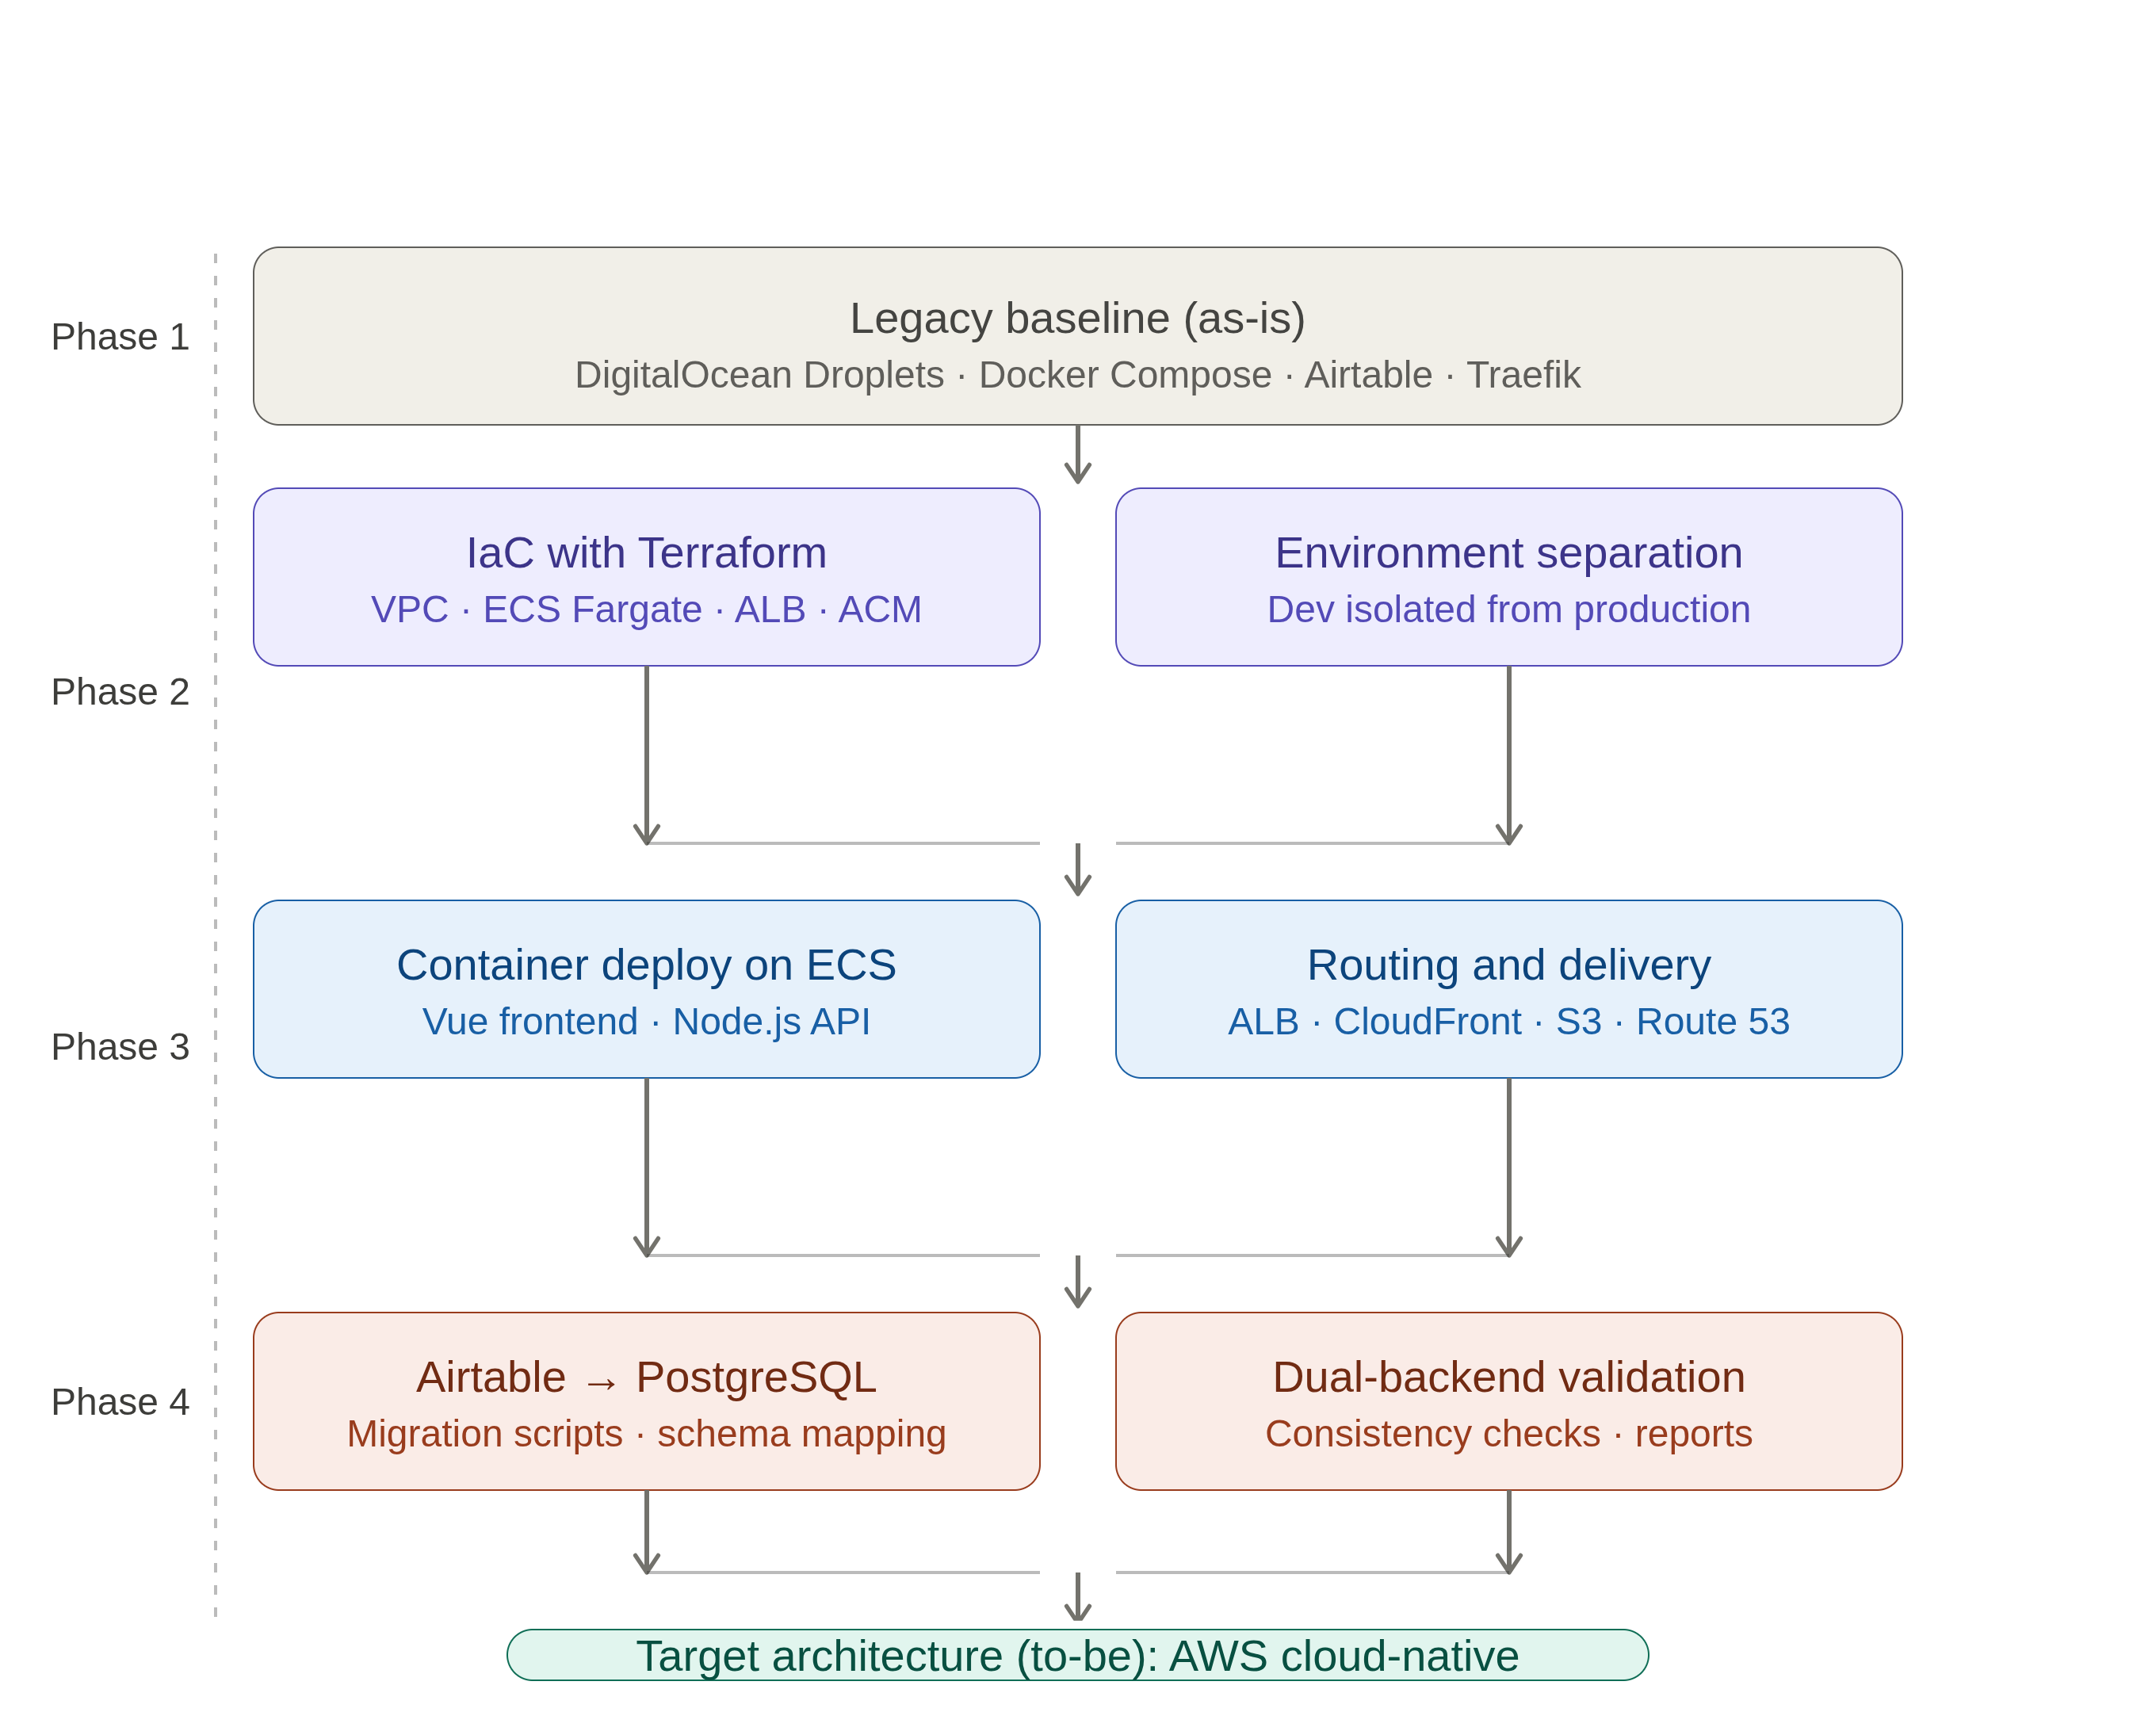
\includegraphics[width=0.95\textwidth]{immagini/migration_incremental_flow_en.png}
    \caption{Incremental execution flow from the legacy baseline to the target AWS cloud-native architecture}
    \label{fig:migration-incremental-flow}
\end{figure}

\section{Infrastructure as Code and Environment Separation}
Infrastructure as Code (IaC) is a software engineering approach in which infrastructure is provisioned and managed through code instead of manual procedures~\cite{awsIacWhitepaper}. Infrastructure definitions become declarative artifacts stored in version control, replacing fragile practices based on manual console operations or ad-hoc scripts and improving consistency and reliability~\cite{awsIacWhitepaper}. Morris identifies three mutually reinforcing core practices: defining everything as code, continuously testing and delivering all work in progress, and building small loosely coupled pieces~\cite{morris2021iac}. A key characteristic is that engineers define the desired final state while automation computes and executes the required operations, providing consistency across environments, auditable version control, automation, reproducibility, and maintainability. In the Outsight Cloud migration, IaC was adopted to automate AWS provisioning and reduce manual intervention during environment setup and updates.

\subsection{Terraform-Driven Provisioning}
Terraform is an IaC tool by HashiCorp that enables provisioning and lifecycle management of infrastructure through declarative configuration files (HCL) that can be versioned, reviewed, and integrated into delivery workflows~\cite{hashicorpTerraformIntro}. It interacts with platforms through providers; in this migration, the AWS provider managed ECS Fargate services, Application Load Balancers, Route~53 records, ACM certificates, VPC networking, S3 storage, and observability infrastructure.

\begin{lstlisting}[language={},caption={Simplified ECS Fargate service definition},label={lst:terraform-ecs}]
resource "aws_ecs_service" "backend" {
  name            = "outsight-backend"
  cluster         = aws_ecs_cluster.main.id
  task_definition = aws_ecs_task_definition.backend.arn

  desired_count = 1
  launch_type   = "FARGATE"

  network_configuration {
    subnets          = aws_subnet.public[*].id
    security_groups  = [aws_security_group.ecs.id]
    assign_public_ip = true
  }
}
\end{lstlisting}

Listing~\ref{lst:terraform-ecs} shows a simplified resource definition used to deploy a backend container as an ECS Fargate service: through declarative configuration, containerized workloads previously orchestrated with Docker Compose could be provisioned reproducibly in AWS while preserving the same packaging model. The Terraform workflow follows three phases~\cite{hashicorpTerraformIntro}: \emph{write} (define the target state declaratively), \emph{plan} (compare desired and current state, showing which resources will be created, updated, or removed), and \emph{apply} (execute the planned operations respecting resource dependencies). This workflow was especially useful for migration safety, since planned changes could be reviewed before execution and applied incrementally. Terraform also keeps a state representation of real infrastructure (\texttt{terraform.tfstate}) to compute incremental changes and detect drift~\cite{hashicorpTerraformIntro}. Terraform was selected because it aligned with the migration objectives: versioned infrastructure definitions, automation integrated into CI/CD processes, reproducible environments, incremental changes, and modular maintainable definitions.

A dedicated effort was made to separate development and production concerns through environment-specific configuration and controlled evolution of shared resources. This separation was particularly important during migration because it allowed AWS environments to be validated independently before production workloads were progressively redirected to the new platform.

\section{Infrastructure Migration Execution}
\label{sec:infra-migration-exec}
While Chapters~\ref{chap:baseline} and~\ref{chap:architecture} describe the legacy platform and target design, this section documents how the transition was executed. The objective was to replace the previous Docker Compose and Traefik deployment model with a reproducible cloud-native foundation without forcing a simultaneous application and data cutover.

The first step translated the target architecture into an IaC baseline using Terraform, provisioning the main building blocks of the target platform: ECS Fargate services for frontend and backend containers, an Application Load Balancer for public routing, Route~53 records for DNS, ACM certificates for HTTPS, CloudWatch log groups for centralized logging, and S3 together with CloudFront for simulation file storage and delivery. A key difference concerned request routing: whereas the legacy environment used Traefik as reverse proxy and HTTPS entry point, routing responsibilities were transferred to the ALB and defined through listener rules mapping traffic to target groups. The backend service was adapted so that its externally exposed routes aligned with the ALB routing model, with a dedicated health-check endpoint for service probes. Container images were published through the existing private registry, and registry credentials were supplied at runtime through AWS Secrets Manager rather than embedded in IaC artifacts or Terraform state.

Simulation file storage was redesigned around a private S3 bucket fronted by CloudFront, replacing the previous S3-compatible integration with an AWS-native delivery model while keeping the bucket non-public through CloudFront Origin Access Control. Public HTTPS access was enabled through ACM-managed certificates integrated with the ALB and CloudFront, and Route~53 managed DNS records per environment. Once provisioned, validation focused on verifying that the new infrastructure behaved correctly before redirecting production traffic, covering ECS service startup, ALB routing, HTTPS and DNS configuration, centralized logging, and the S3/CloudFront flow. Development and production concerns were kept separated so that experimental changes and database modernization could be isolated from the production system still running on the legacy platform. The final transition consisted of progressively redirecting public access from the legacy environment to AWS through DNS updates in Route~53, avoiding a single disruptive cutover across infrastructure, routing, and data storage simultaneously.

\section{Data Migration Tooling and Validation}
The migration path from Airtable to PostgreSQL was implemented with schema and migration tooling designed to preserve compatibility constraints, aiming not only at data transfer but at controlled evolution toward explicit schema ownership. Dedicated scripts were developed to replicate data from Airtable into PostgreSQL, validate consistency through machine-readable reports, and verify migration correctness at each checkpoint before production switchover. These artifacts transformed data migration from a one-time operation into a repeatable and verifiable workflow, providing measurable confidence in the correctness of the transition before the final cutover.
